\documentclass[problem]{mcs}

\begin{pcomments}
  \pcomment{CP_pythagorean}
  \pcomment{ARM 01/24/15 from welcome slides}
\end{pcomments}

\pkeywords{
   pythagorean
   triangle
   square
}

%%%%%%%%%%%%%%%%%%%%%%%%%%%%%%%%%%%%%%%%%%%%%%%%%%%%%%%%%%%%%%%%%%%%%
% Problem starts here
%%%%%%%%%%%%%%%%%%%%%%%%%%%%%%%%%%%%%%%%%%%%%%%%%%%%%%%%%%%%%%%%%%%%%

\begin{problem}

\begin{figure}[h]
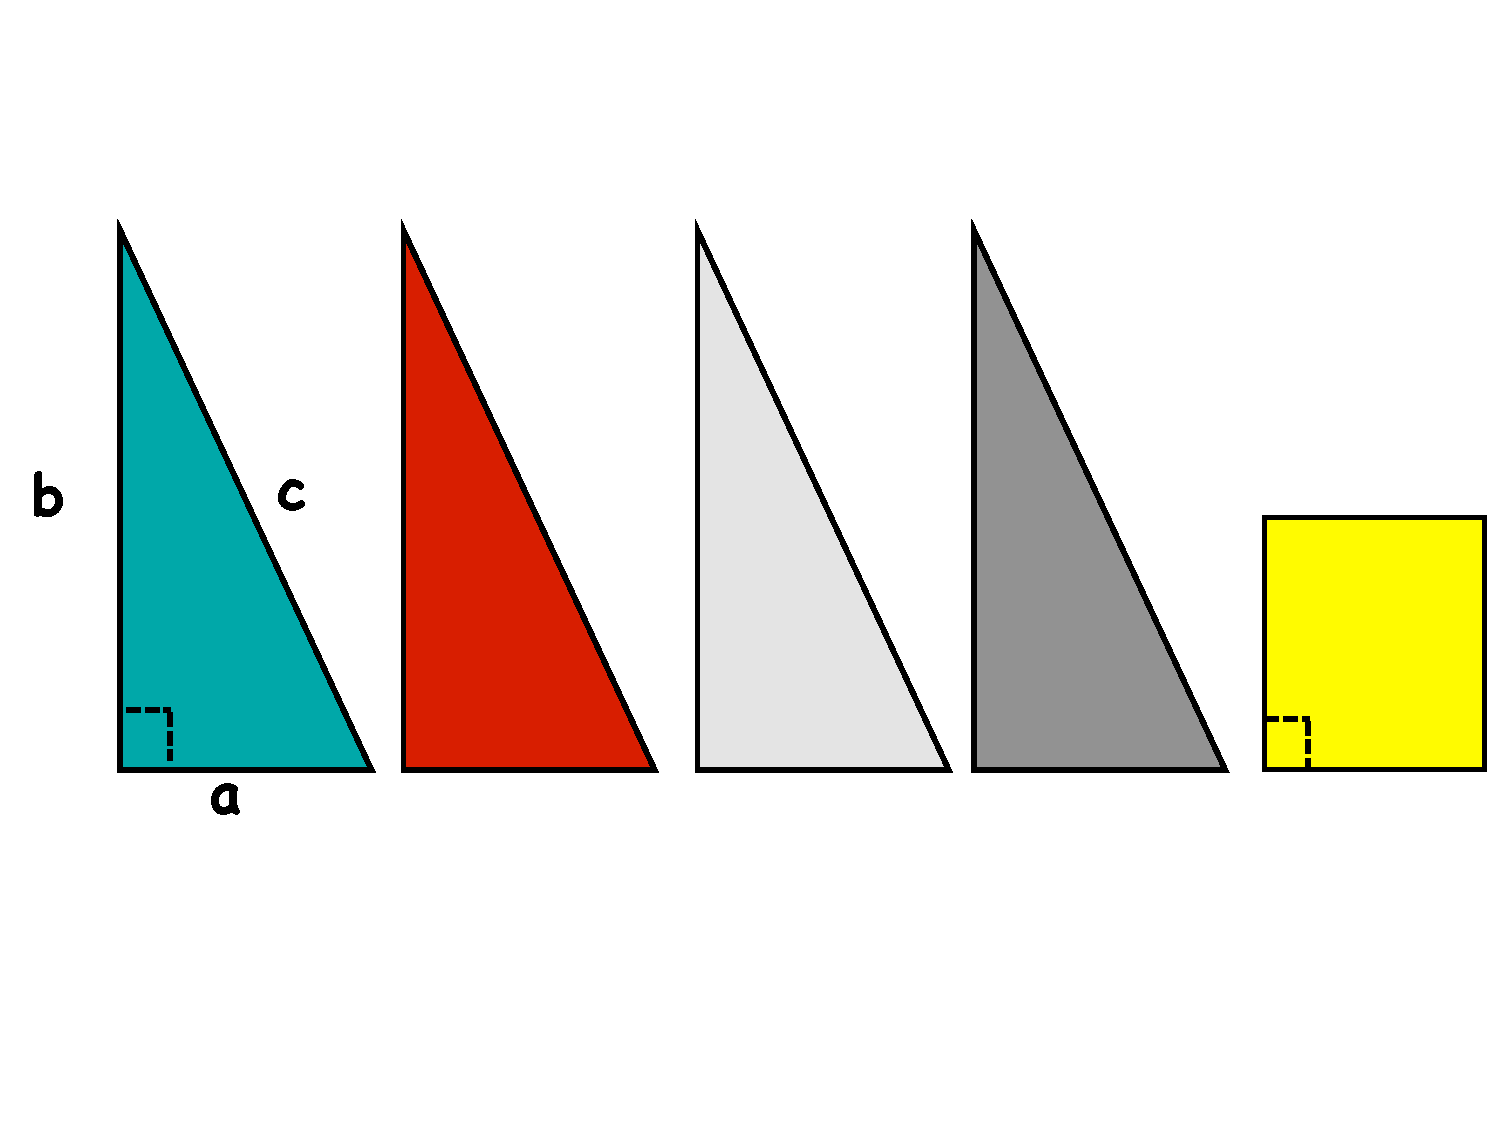
\includegraphics[width=\linewidth]{pythagorean-triangles}
\caption{Right triangles and square.}
\label{fig:righttri}
\end{figure}



\begin{figure}[h]
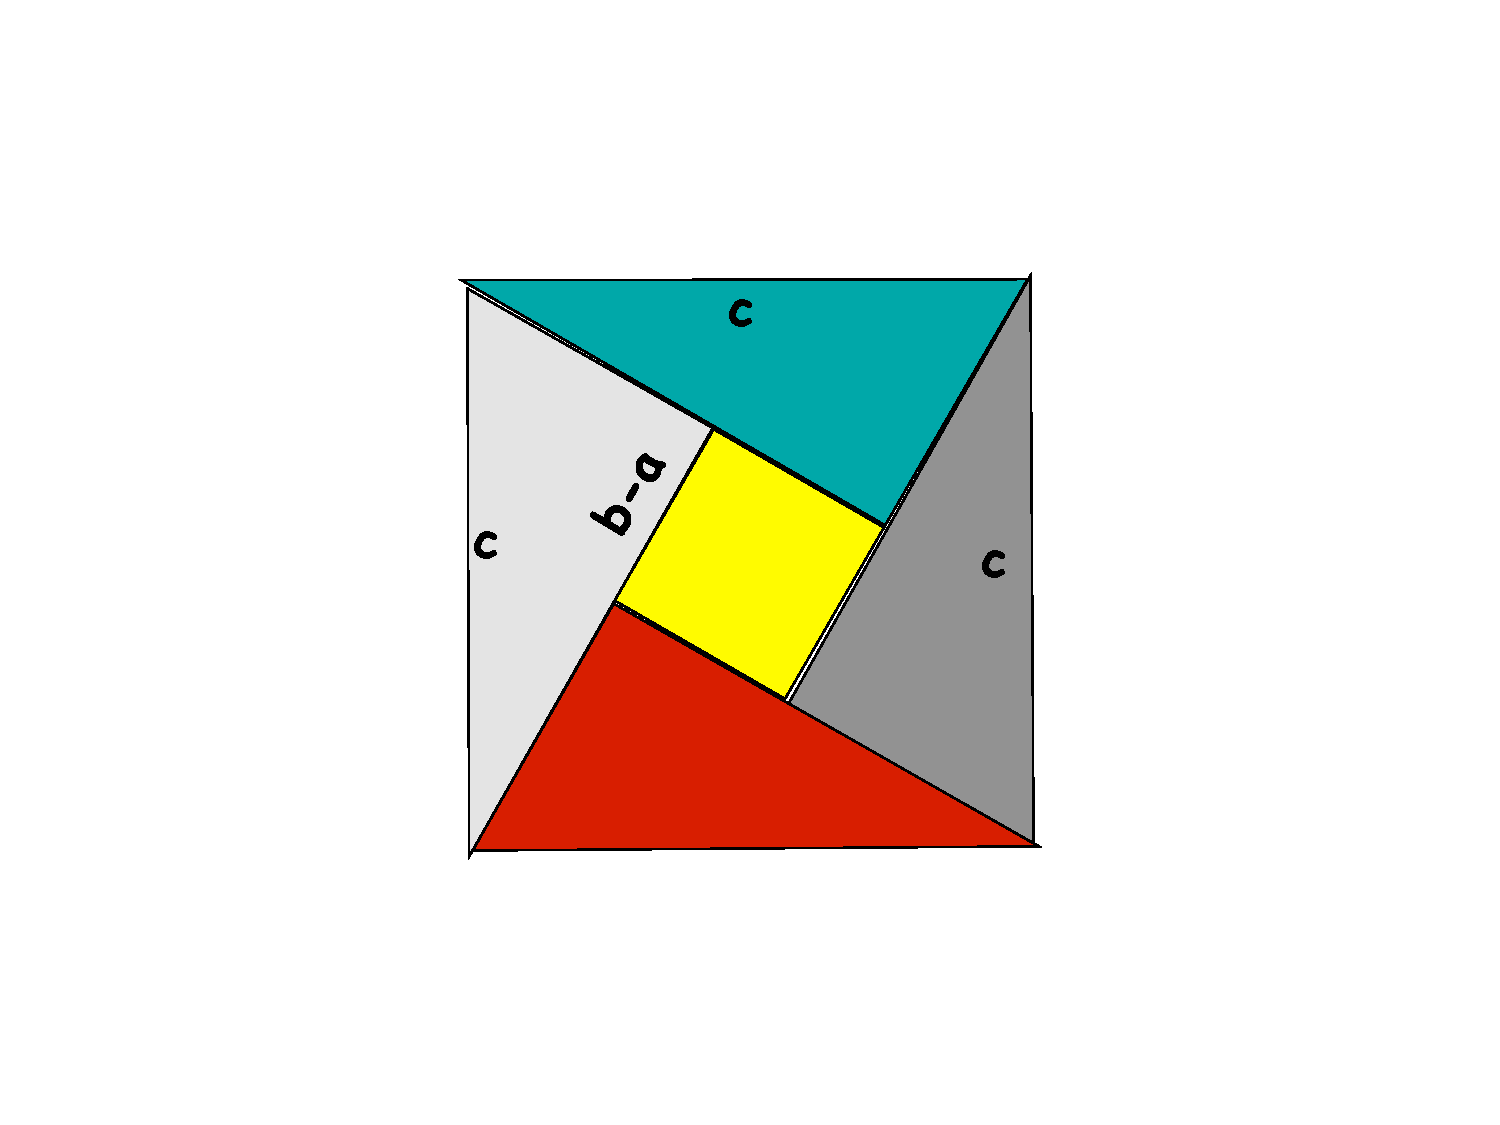
\includegraphics[width=1.2\linewidth]{cxc-arrangement}
\caption{$c \times c$ square.}
\label{fig:cxcsq}
\end{figure}


\begin{figure}[h]
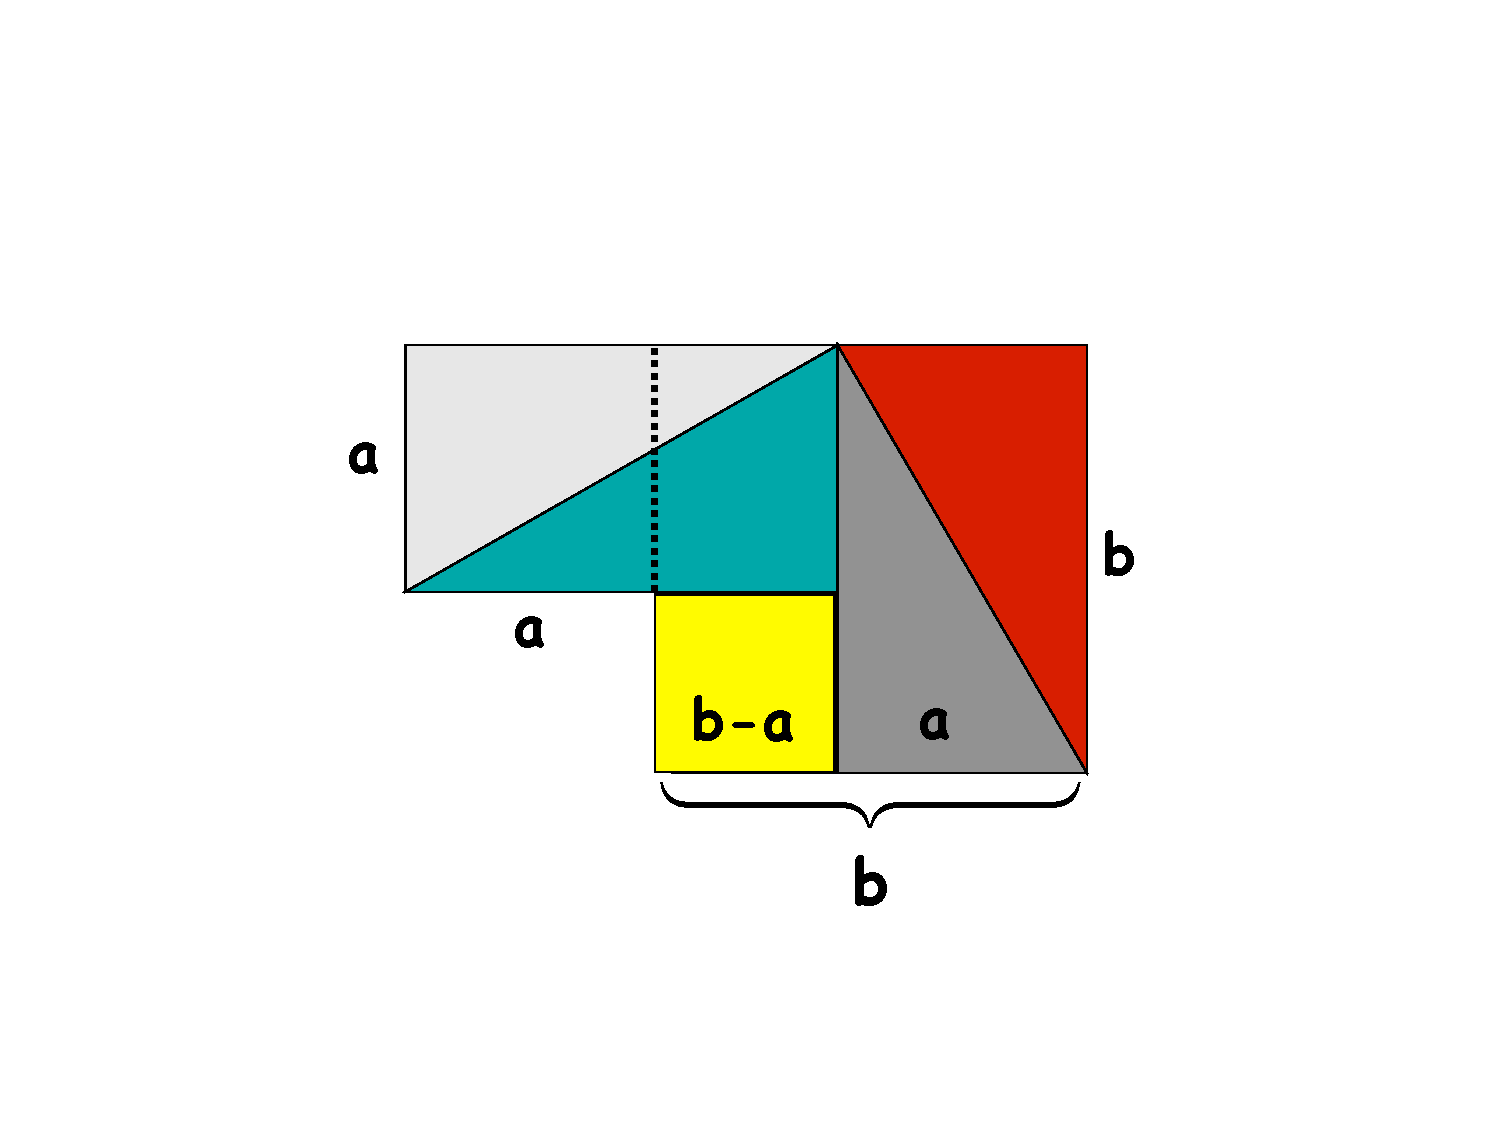
\includegraphics[width=1.2\linewidth]{axa_bxb_arrangement}
\caption{$a \times a$ and $b \times $ squares.}
\label{fig:axabxb}
\end{figure}

 
\end{problem}

%%%%%%%%%%%%%%%%%%%%%%%%%%%%%%%%%%%%%%%%%%%%%%%%%%%%%%%%%%%%%%%%%%%%%
% Problem ends here
%%%%%%%%%%%%%%%%%%%%%%%%%%%%%%%%%%%%%%%%%%%%%%%%%%%%%%%%%%%%%%%%%%%%%

\endinput
